\documentclass[letterpaper]{article}
\usepackage{geometry}
\geometry{letterpaper, portrait, margin=.8in,top=1in}
\usepackage[english]{babel}
\usepackage[utf8]{inputenc}
\usepackage{amsmath}
\usepackage{graphicx}
\usepackage[backend=biber]{biblatex}
\usepackage{hyperref}
\usepackage{listings}
\usepackage{color}
\definecolor{dkgreen}{rgb}{0,0.6,0}
\definecolor{gray}{rgb}{0.5,0.5,0.5}
\definecolor{mauve}{rgb}{0.58,0,0.82}
\lstset{frame=tb,
  language=C++,
  aboveskip=3mm,
  belowskip=3mm,
  showstringspaces=false,
  columns=flexible,
  basicstyle={\small\ttfamily},
  numbers=none,
  numberstyle=\tiny\color{gray},
  keywordstyle=\color{blue},
  commentstyle=\color{dkgreen},
  stringstyle=\color{mauve},
  breaklines=true,
  breakatwhitespace=true,
  tabsize=3
}
\bibliography{ROOT0908}
\title{PHYS-592 Mid-Term}
\author{Jason Wyenberg}
\begin{document}
\maketitle
\begin{abstract}
The PHYS-592 Mid-Term is upon us!
\end{abstract}
\section{Trees with ROOT}
\subsection{Energy Spectrum}
Figure \ref{Figure1} below shows the energy spectrum from the data.
\begin{figure}[htpb]
  \centering
  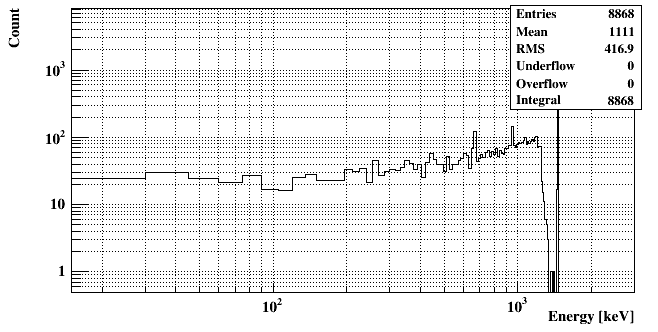
\includegraphics[width=.8\linewidth]{Figure1}
  \caption{Energy Spectrum}
  \label{Figure1}
\end{figure}
\subsection{Normalized Energy Spectrum}
Figure \ref{Figure2} below shows the normalized energy spectrum from the data, with a gaussian fit.
\begin{figure}[htpb]
  \centering
  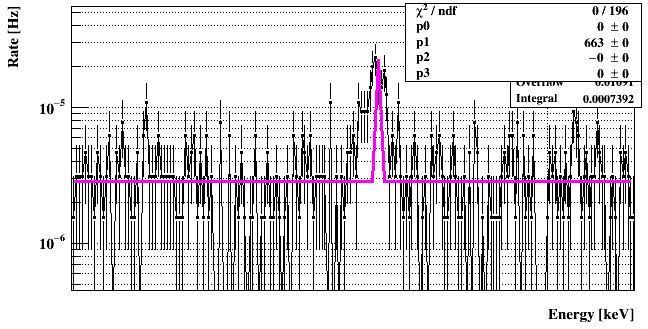
\includegraphics[width=.8\linewidth]{Figure2}
  \caption{Normalized Energy Spectrum}
  \label{Figure2}
\end{figure}
\subsection{Distribution}
Figure \ref{Figure3} below shows the distribution of events. It looks like the detector is a spherical shape based on the distribution plot.
\begin{figure}[htpb]
  \centering
  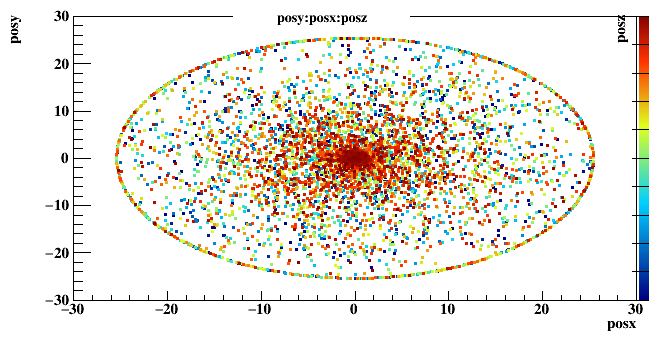
\includegraphics[width=.8\linewidth]{Figure3}
  \caption{Normalized Energy Spectrum}
  \label{Figure3}
\end{figure}
\subsection{The code that was used}
The following code was written as a script for Root:
\begin{lstlisting}
// C file that builds a tree and generates a histogram of the data from Jing's energy data.txt file

void exam(){

//Declare variables

  Float_t    energy;
  Float_t    posx;
  Float_t    posy;
  Float_t    posz;

//Create new files
  TFile *f = new TFile("exam.root","RECREATE");
  
  FILE *fp = fopen("data.txt","r");
//fopen opens oil.dat. "r" means read and write
  
  TTree *tree = new TTree("T","Jing's Exam data");
  tree->Branch("energy",&energy,"energy/F");
  tree->Branch("posx",&posx,"posx/F");
  tree->Branch("posy",&posy,"posy/F");
  tree->Branch("posz",&posz,"posz/F");
  
  char line[8900];    //number of entries must be greater than the amount of lines
  while (fgets(&line,8900,fp)) {
    sscanf(&line[0], "%g %g %g %g",&energy,&posx,&posy,&posz);
    tree->Fill();
  }
  
  tree->Print();
  tree->Write();
  
  TCanvas *can = new TCanvas;
  can->Divide(2,2);
//  can->cd(1);
//  T->Draw("energy:posx:posy","posy<25","colz");
  
  TH1F *henergy = new TH1F("hnenergy",";energy", 200, 0, 3000);

  int n = (Int_t)T->GetEntries();
  for (Int_t i=0; i<n; i++)  {
    T->GetEntry(i);
    henergy->Fill(energy);
  }
  
  can->cd(1)->SetLogy();
  can->cd(1)->SetLogx();
  can->cd(1)->SetGridy();
  can->cd(1)->SetGridx();
  henergy->GetYaxis()->SetTitle("Count");
  henergy->GetXaxis()->SetTitle("Energy [keV]");
  henergy->Draw();

  TH1F *hnenergy = (TH1F*) henergy->Clone();
//  hnenergy->SetName("hnenergy");
//  hnenergy->GetXaxis()->SetRange(600,720);   //this does not seem to be working for me
  
  TH1F *hnenergy2 = new TH1F("hnenergy2",";energy", 200, 600, 720);

  int n = (Int_t)T->GetEntries();
  for (Int_t i=0; i<n; i++)  {
    T->GetEntry(i);
    hnenergy2->Fill(energy);
  }

  hnenergy2->Sumw2();
  
  can->cd(2)->SetLogy();
  can->cd(2)->SetLogx();
  can->cd(2)->SetGridy();
  can->cd(2)->SetGridx();
  float scale_factor = 3*60*3600;
  hnenergy2->Scale(1./scale_factor);
  hnenergy2->GetYaxis()->SetTitle("Rate [Hz]");
  hnenergy2->GetXaxis()->SetTitle("Energy [keV]");
  hnenergy2->Draw("e");
  
  TF1 *fc = new TF1("fc","[3]+gaus(0)",0,8500);
  fc->SetParameters(.0001,680.,20.,.000005);
  fc->SetLineColor(kMagenta);
  TGraph *gr = new TGraph(hnenergy2);
  gr->SetTitle("Fit");
  gr->Fit("fc");
  gr->Draw("same");
  
  can->cd(3);
  T->Draw("posy:posx:posz","","colz");
  
  hnenergy->Print();
  hnenergy->Write();
  
}
\end{lstlisting}
\newpage
\printbibliography 
\end{document}
